%!TEX root = ../thesis.tex
%*******************************************************************************
%****************************** Third Chapter **********************************
%*******************************************************************************
\chapter{Pengujian dan Analisa Sistem}

% **************************** Define Graphics Path **************************
\ifpdf
    \graphicspath{{Chapter4/Figs/tinggi/}{Chapter4/Figs/idv/}{Chapter4/Figs/}}
\else
    \graphicspath{{Chapter4/Figs/Vector/}{Chapter4/Figs/}}
\fi

Pada bab ini menjelaskan mengenai proses pengujian dan hasil yang didapat dari pengujian tersebut. Pengujian kali ini mencakup dari pengambilan gambar, pengiriman hingga tedeksi korban bencana alam menggunakan berbagai sumber gambar.

\section{Pengujian Pengambilan dan Pengiriman Gambar}

\begin{figure}[ht]
  \centering
  \begin{subfigure}[b]{0.495\textwidth}
    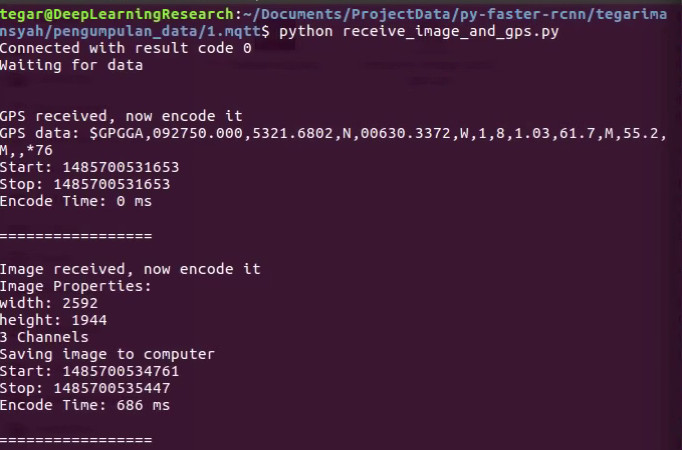
\includegraphics[width=\textwidth]{mqtt_server}
    \caption{}
  \end{subfigure}             
  \begin{subfigure}[b]{0.495\textwidth}
    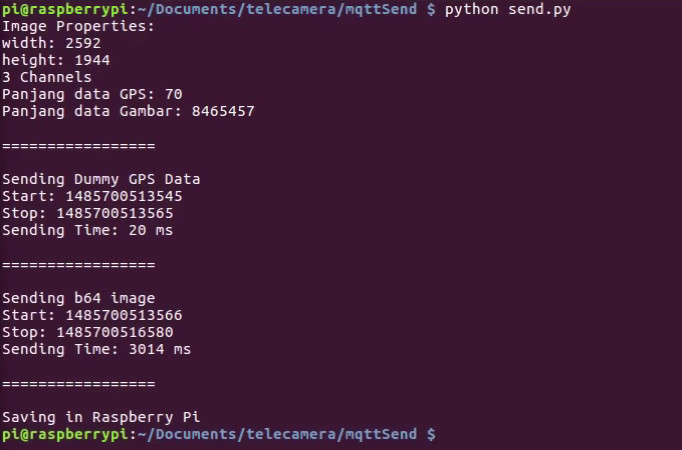
\includegraphics[width=\textwidth]{mqtt_raspi}
    \caption{}
  \end{subfigure}
 \caption{Protokol MQTT Dijalankan Pada Server (a) dan Raspberry Pi (b)}
 \label{fig:mqtt_result}   
\end{figure}

Pada pengujian kali ini dilakukan pengambilan gambar dan pengiriman gambar dari Raspberry Pi 3 menuju komputer perangkat pengolahan data. Kamera yang digunakan adalah RaspiCam 1.3 dan pengambilan gambar dilakukan dengan varian resolusi untuk mengetahui ukuran dan kecepatan gambar. Raspberry Pi dijalankan secara \textit{remote} pada komputer. Pada Gambar~\ref{fig:mqtt_result} diperlihatkan dua buah window dimana yang window kanan sedang melakukan \textit{remote} menjalankan proses pengambilan dan pengiriman gambar oleh Raspberry Pi sedangkan window kiri menunggu dan menerima gambar pada komputer. Kedua program tersebut memberikan informasi gambar seperti \textit{width, height, channels, } waktu mulai selesai transfer data. Percobaan dilakukan dengan empat resolusi gambar yang berbeda dan disajikan pada tabel berikut.

\begin{table}[ht]
\centering
\caption{Tabel Pengukuran Kecepatan Pengiriman dan Penerimaan Gambar}
\label{table:mqtt}
\resizebox{\textwidth}{!}{%
\begin{tabular}[\textwidth] { c c c c}
\hline 
Resolution & Data Size & Sending Time & Encoding Time \\
(WxH) & (Bytes) & (ms) & (ms) \\
\hline
640 x 480 & 0.478.377 &  0266 & 070 \\
800 x 600 & 0.749.899 & 0282 & 051 \\
1296 x 972 & 2.589.624 & 0987 & 203 \\
2592 x 1944 & 8.465.457 & 3014 & 686 \\
\hline 
\end{tabular} }
\end{table}

Pada Tabel~\ref{table:mqtt}, diperlihatkan rata-rata ukuran data, rata-rata waktu pengiriman dan rata-rata waktu \textit{encode} yang ada pada masing masing resolusi. Seperti dijelaskan pada bab sebelumnya, proses pengiriman gambar dilakukan dengan cara mengambil gambar lalu diubah menggunakan \textit{string base64} sehingga diperoleh ukuran data tersebut. Peningkatan ukuran data dari resolusi 640x480 ke 800x600 sekitar 1,57 kali, 800x600 ke 1296x972 sekitar 3,45 kali dan 1296x972 ke 2592x1944 sekitar 3,27 kali. Sedangkan waktu yang dibutuhkan untuk mengirimkan data masing masing sebesar 1,06 , 3,5 dan 3,05 detik. Hal menarik terdapat pada kolom waktu \textit{encode} dimana waktu yang dibutuhkan oleh resolusi 800x600 lebih cepat dari pada resolusi 640x480.


\section{Pengujian Learning dan Testing Berbagai Net}

Pada pengujian kali ini dilakukan learning dan testing dari tiga buat Net yaitu VGG16, VGG CNN M 1024 dan ZF. Net tersebut dibangun diatas caffe dan diberikan metode Faster R-CNN untuk meningkatkan akurasi. Pengujian ini dijalankan pada komputer pengolahan data. Proses learning dan testing menggunakan Dataset PASCAL VOC 2007. Hasil yang didapatkan dapat dilihat pada Tabel~\ref{table:learning}.

\begin{table}[ht]
\centering
\caption{Tabel Pengukuran Kecepatan Learning dan Testing}
\label{table:learning}
\resizebox{\textwidth}{!}{%
\begin{tabular}[\textwidth] { c c c c c c }
\hline 
Net & Waktu per & \multicolumn{2}{c}{Waktu} &  AP & Waktu Deteksi \\
& Iterasi & Learning & Testing & & (s/image) \\
\hline
VGG16 & 0,313s &366m 39,835s & 7m 21,173s & 0,2790 & 0,085 \\
VGG CNN M 1024 & 0,072s & 084m 15,170s & 3m 53,005s & 0,2429 & 0,042 \\
ZF & 0.148s &172m 56,947s & 3m 06,899s & 0,2442 & 0,035 \\
\hline 
\end{tabular} }
\end{table}

Dari tabel di atas, dapat dilihat waktu yang dibutuhkan dalam satu iterasi, waktu total proses learning, waktu total proses testing dan waktu deteksi pergambar serta Avarage Precision (AP). VGG16 membutuhkan waktu per iterasi paling lama dengan nilai 0,313 detik, dimana ZF hanya membutuhkan 0,148 detik dan VGG CNN M 1024 hanya 0,072 detik. Total waktu yang dibutuhkan VGG16 untuk proses learning sekitar 6,1 jam, dimana ZF membutuhkan waktu sekitar 2,87 jam dan VGG CNN M 1024 hanya 1,4 jam. Hasilnya dapat dilihat pada AP menggunakan dataset tersebut dimana VGG16 memiliki nilai tertinggi yaitu 0,279, sedangkan ZF memiliki nilai 0,0013 lebih presisi. Untuk kecepatan deteksi gambar, ZF memiliki waktu tercepat dimana hanya membutuhkan waktu 0,035 detik per gambar. Dari ketiga Net tersebut, masing masing menghasilkan model yang dapat digunakan untuk melakukan proses deteksi.

\section{Pengujian Deteksi Manusia Menggunakan IDV-50}

Pada pengujian kali ini dilakukan deteksi manusia dari kumpulan gambar IDV-50 menggunakan model ZF. IDV-50 merupakan kumpulan gambar yang terdiri dari 50 gambar manusia dengan latar belakang bencana. Hasil deteksi mengikuti format seperti dijelaskan pada Gambar~\ref{fig:fotmat_deteksi}. Hasil deteksi dapat dilihat pada Gambar~\ref{fig:korban_bencana_idv}.

\begin{figure}[ht]
 \centering
 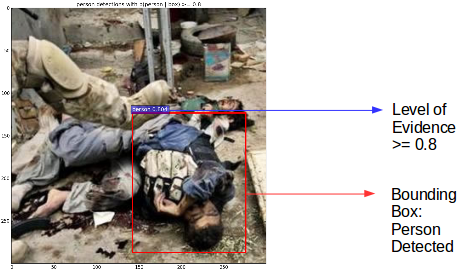
\includegraphics[width=0.8\textwidth]{format_deteksi}
 \caption{Format Deteksi}
 \label{fig:fotmat_deteksi}   
\end{figure}

Ketika pada sebuah gambar terdeteksi manusia, maka akan secara otomatis dibentuklah sebuah \textit{bounding box} berwarna merah yang menandainya yang merupakan hasil perhitungan dari \textit{bbox score}. Sebuah objek dikatakan terdeteksi jika melewati \textit{treshold confidence} sebesar 0.8 atau $80\%$. Confidence atau tingkat kepercayaan adalah sebuah probabilitas yang dihitung oleh net pada \textit{cls score} yang menggambarkan kesesuaian objek dengan model yang dibuat.

\begin{figure}[ht]
  \centering
  \begin{subfigure}[b]{0.3\textwidth}
    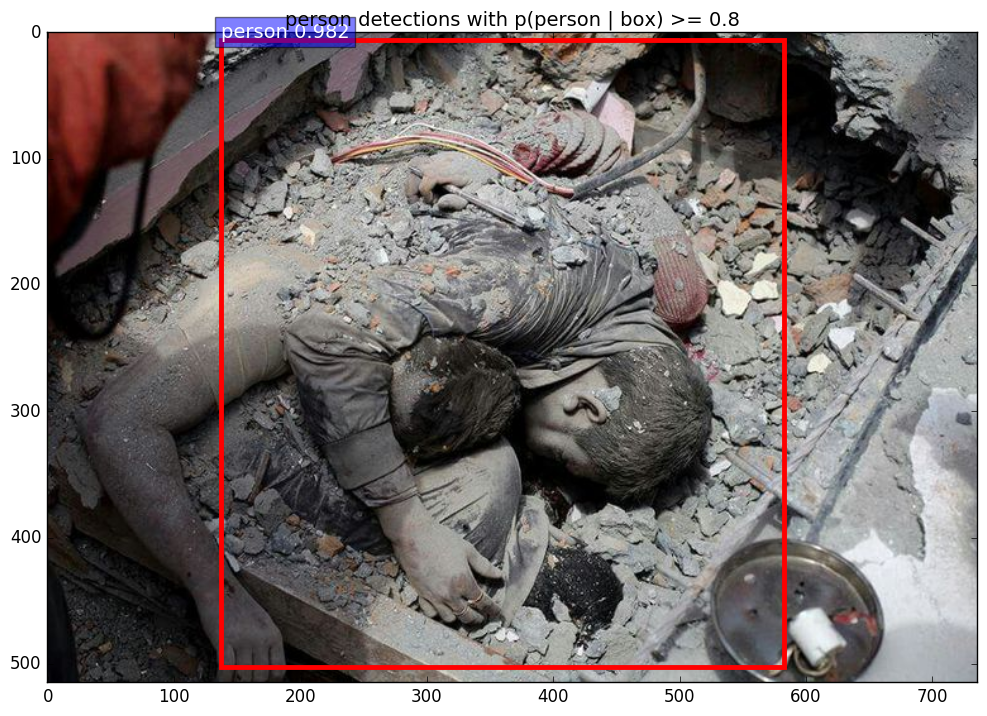
\includegraphics[width=\textwidth]{idv1}
  \end{subfigure}             
  \begin{subfigure}[b]{0.3\textwidth}
    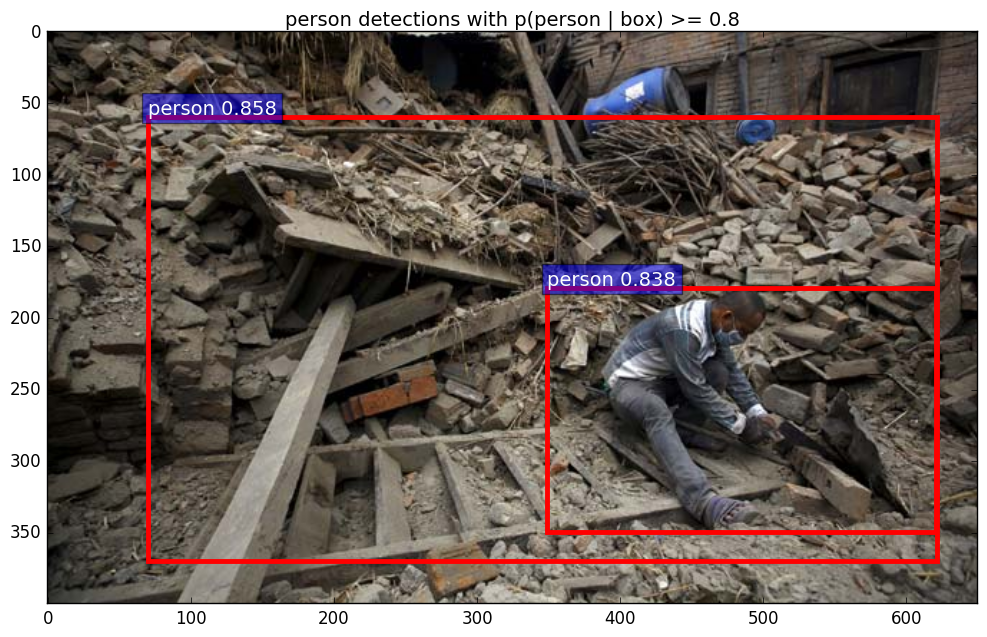
\includegraphics[width=\textwidth]{idv2}
  \end{subfigure}
  \begin{subfigure}[b]{0.3\textwidth}
    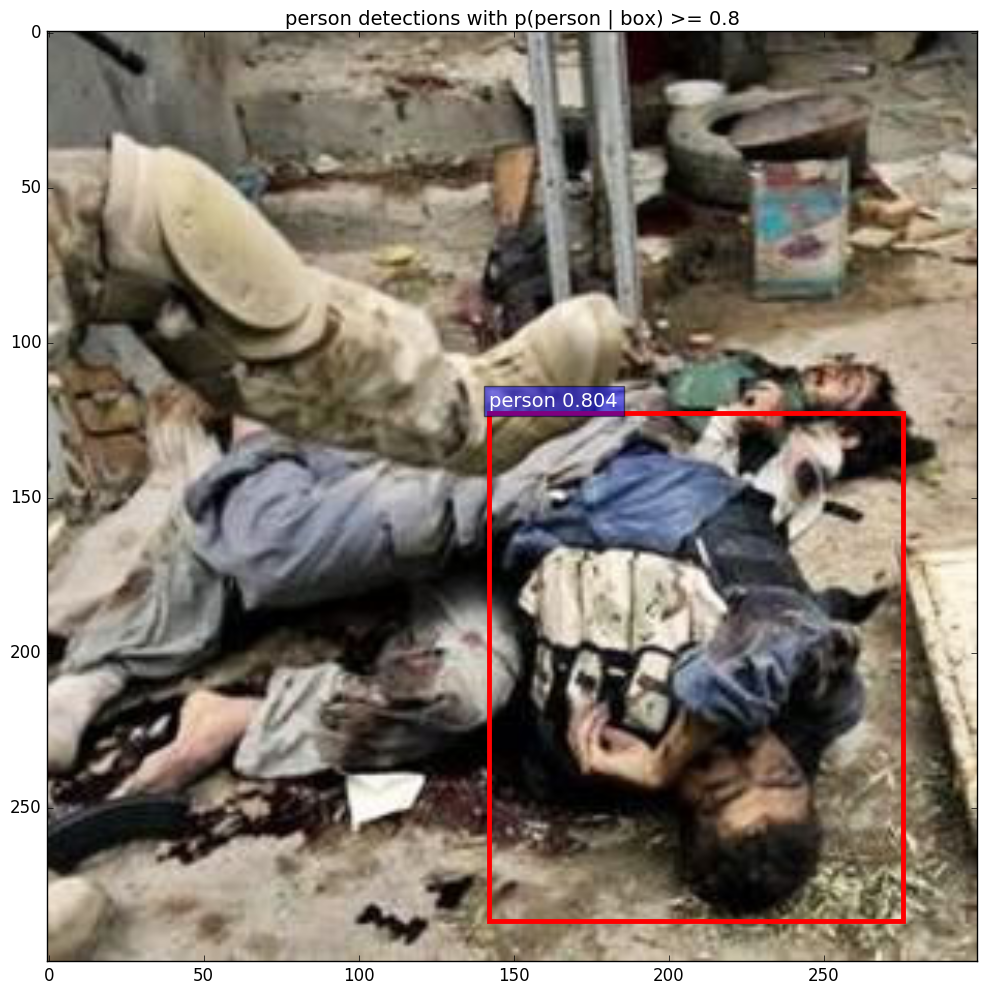
\includegraphics[width=\textwidth]{idv3}
  \end{subfigure}             
  \begin{subfigure}[b]{0.3\textwidth}
    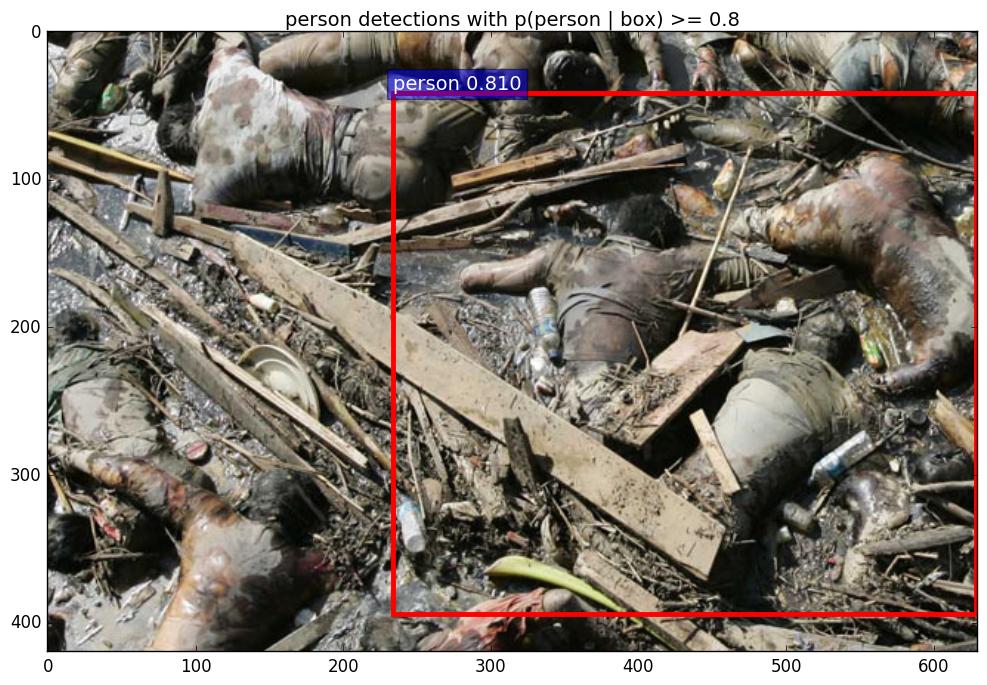
\includegraphics[width=\textwidth]{idv4}
  \end{subfigure}
  \begin{subfigure}[b]{0.3\textwidth}
    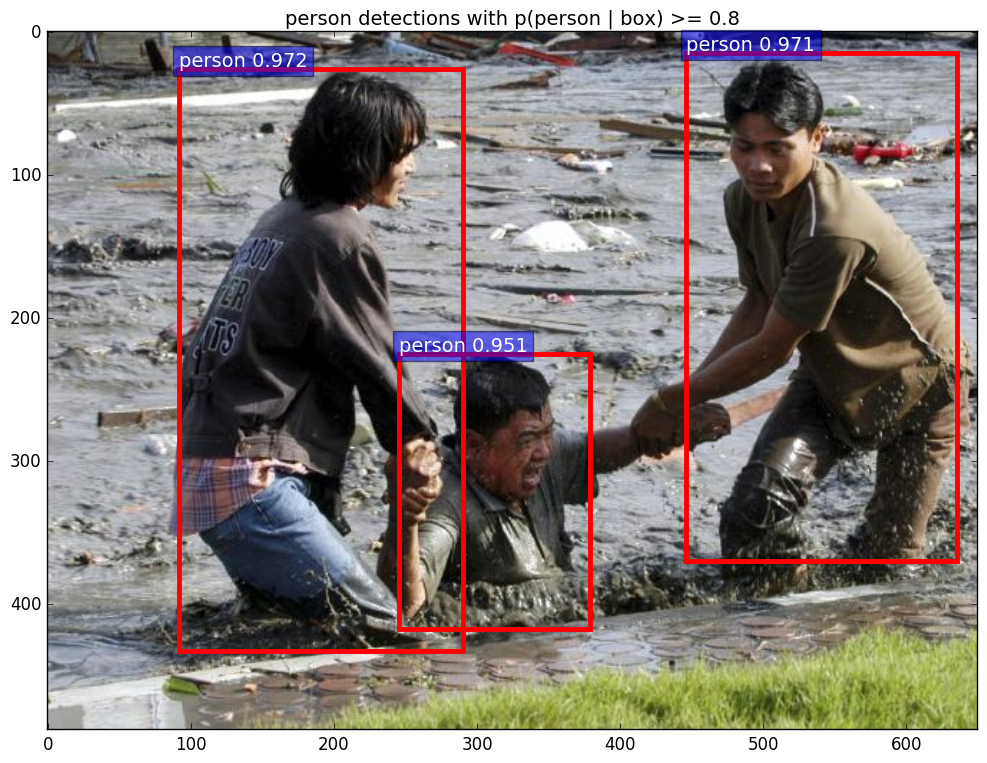
\includegraphics[width=\textwidth]{idv5}
  \end{subfigure}             
  \begin{subfigure}[b]{0.3\textwidth}
    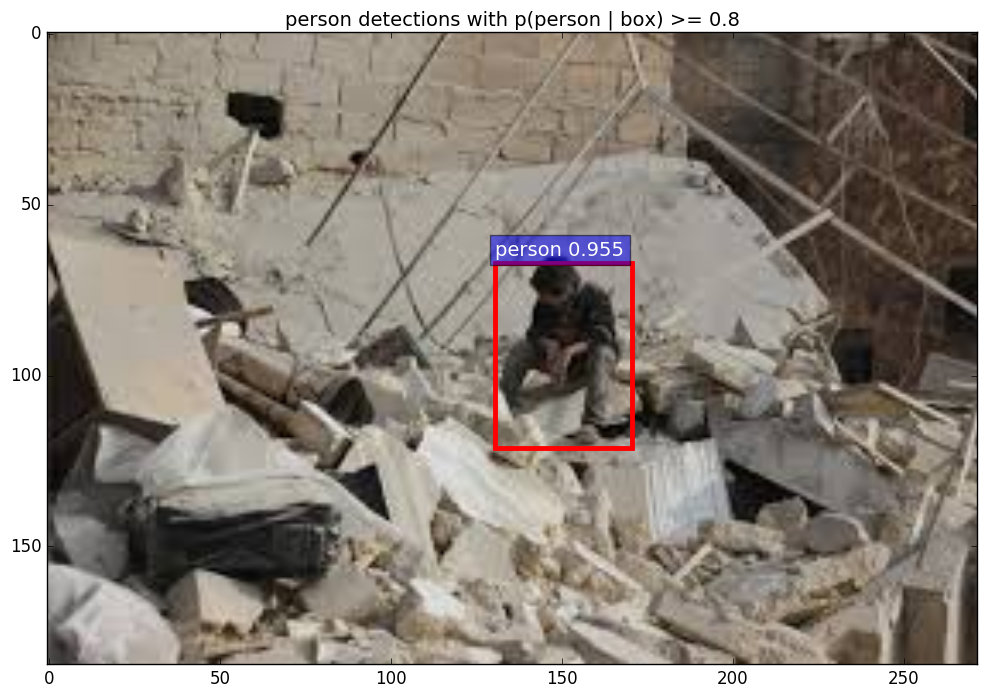
\includegraphics[width=\textwidth]{idv6}
  \end{subfigure}
  \caption{Korban Bencana IDV}
  \label{fig:korban_bencana_idv}
\end{figure}

Dari 50 gambar yang disediakan, model ZF mampu mendeteksi pada 43 gambar. Gambar yang dianggap terdeteksi memiliki nilai AP diatas 0.80 atau dapat dikatakan memiliki tingkat kepercayaan $80\%$. Pada 43 gambar tersebut, terdapat beberapa kondisi dimana hanya beberapa manusia yang terdeteksi dari keseluruhan manusia pada satu gambar. 

\section{Pengujian Deteksi Pada Varian Ketinggian}

Pada pengujian kali ini dilakukan deteksi manusia dengan tiga sikap yaitu terlentang, miring dan tertutup sebagian. Hal ini untuk mengetahui bagaimana hasil deteksi terhadap ketiga gaya tersebut. Pengambilan gambar dilakukan dengan berbagai ketinggian dan berbagai resolusi yang digunakan. Gambar dengan resolusi yang berbeda diambil secara berurutan secara otomatis dalam waktu yang hampir bersamaan sehingga dapat dikatakan sama hanya berbeda resolusi. Pengambilan gambar dilakukan pada pukul 14.00 - 15.00 dengan kondisi cuaca berawan ringan dengan suhu sekitar $32^{\circ}$. Pengambilan gambar menggunakan perangkat Raspberry Pi 3 dan kamera RaspiCam 1.3 di Gedung Pasca Sarjana PENS lantai 1 hingga 6. Hasil pengambilan gambar lalu dilakukan \textit{testing} menggunakan model ZF.

\begin{figure}[ht]
  \centering
  \begin{subfigure}[b]{0.27\textwidth}
    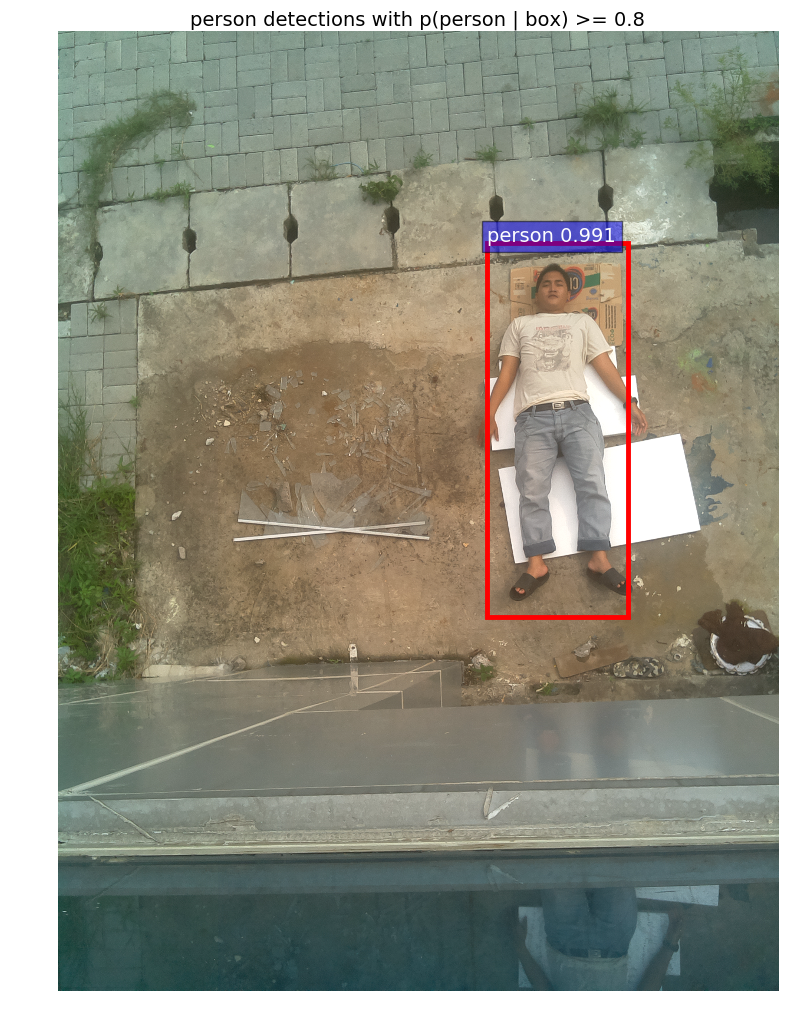
\includegraphics[width=\textwidth]{1}
    \caption{}
  \end{subfigure}             
  \begin{subfigure}[b]{0.27\textwidth}
    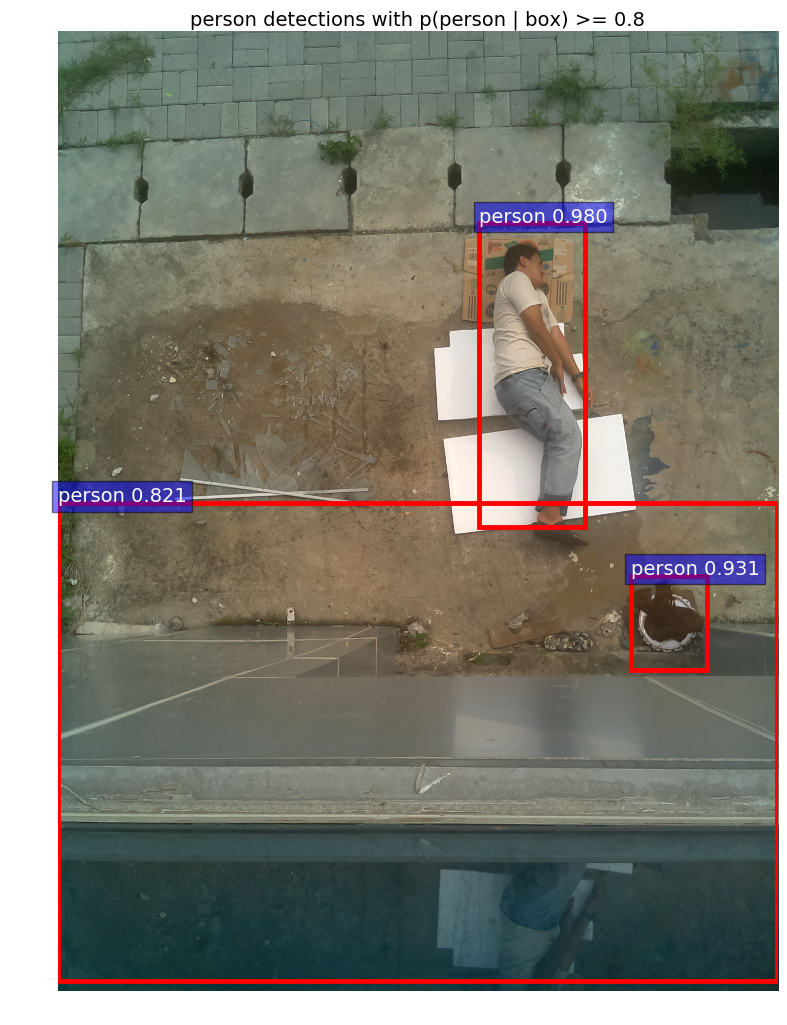
\includegraphics[width=\textwidth]{2}
    \caption{}
  \end{subfigure}
  \begin{subfigure}[b]{0.27\textwidth}
    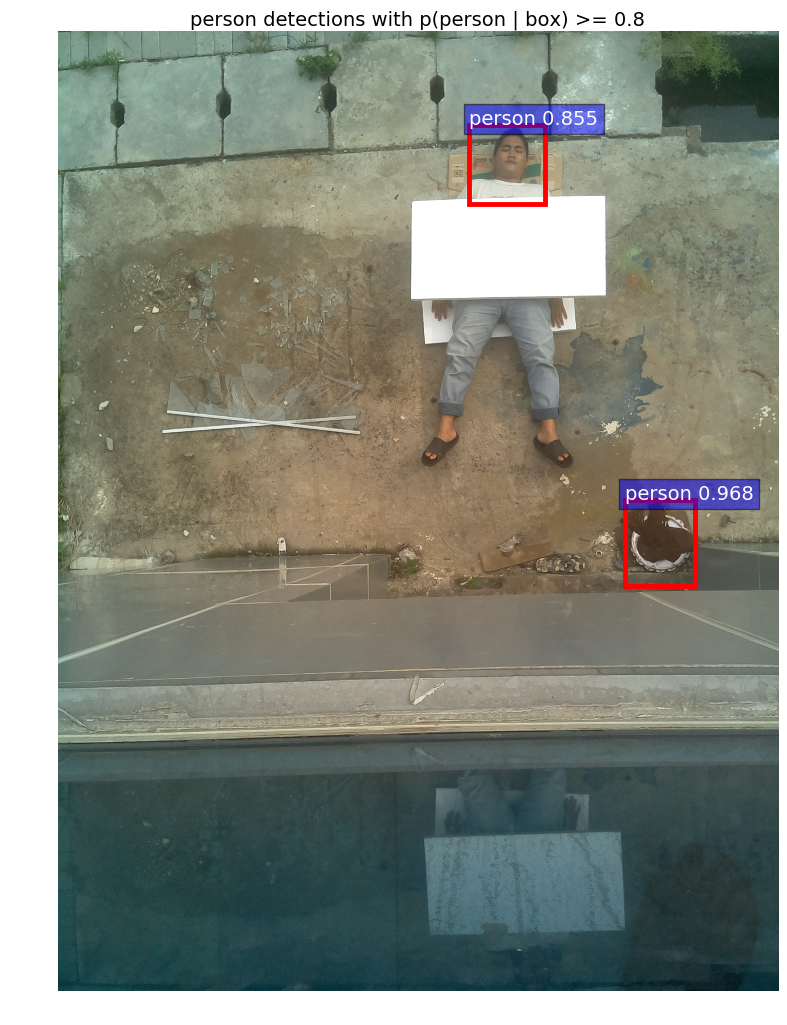
\includegraphics[width=\textwidth]{3}
    \caption{}
  \end{subfigure}             
  \begin{subfigure}[b]{0.27\textwidth}
    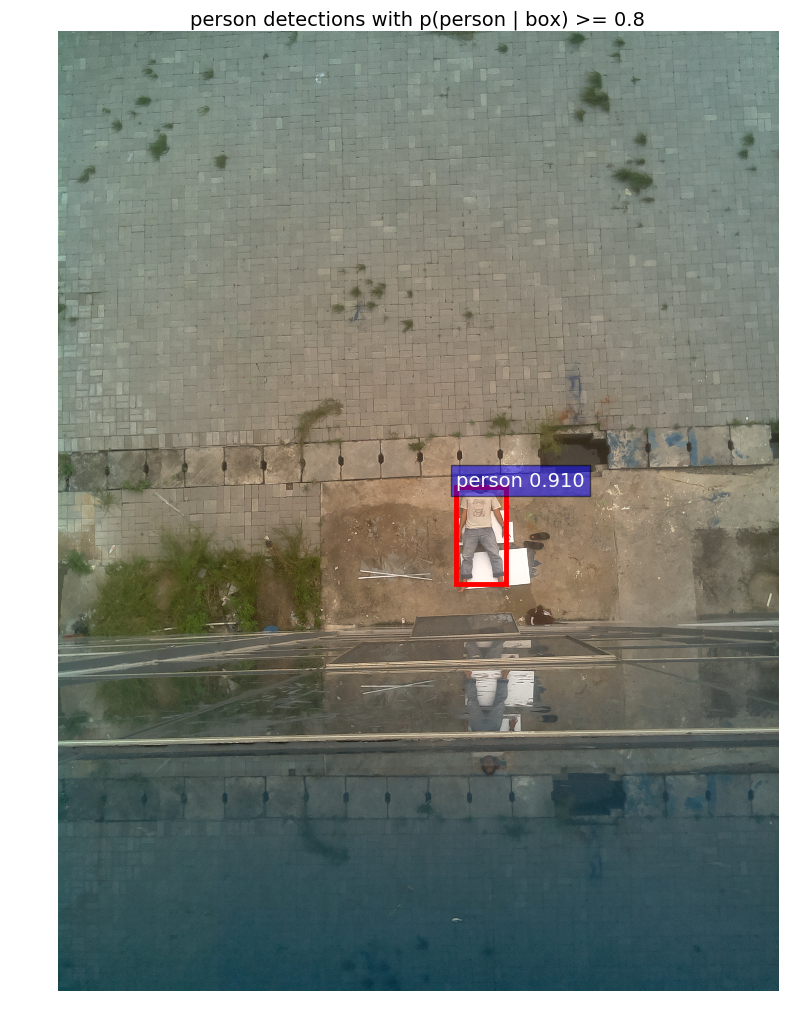
\includegraphics[width=\textwidth]{4}
    \caption{}
  \end{subfigure}
  \begin{subfigure}[b]{0.27\textwidth}
    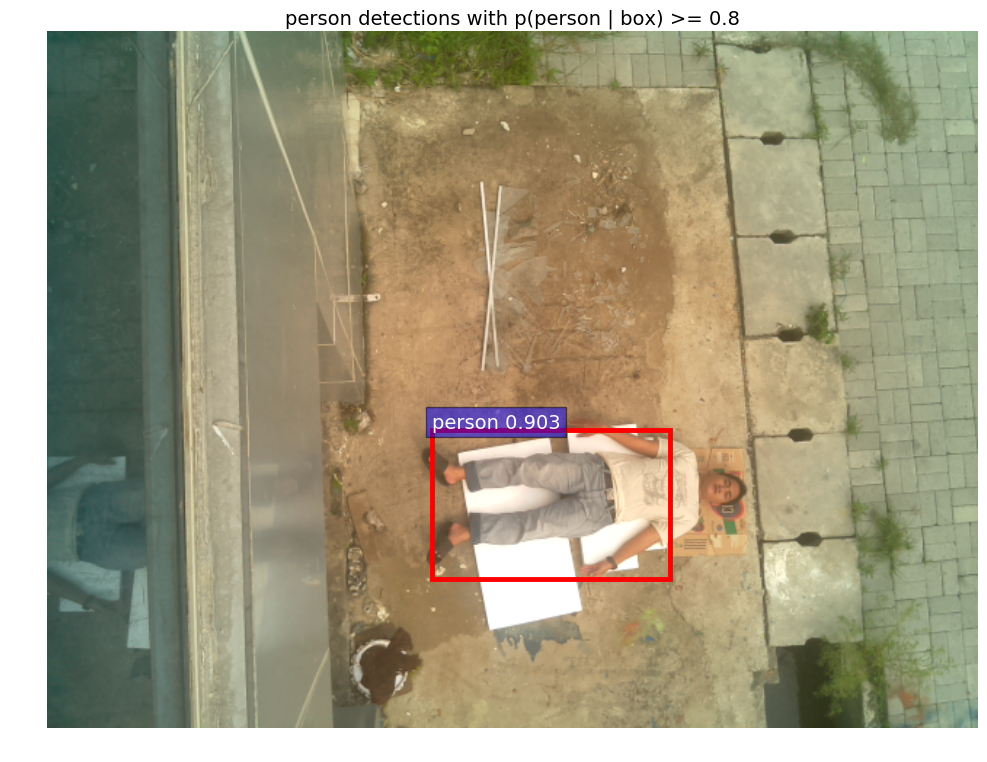
\includegraphics[width=\textwidth]{5}
    \caption{}
  \end{subfigure}             
  \begin{subfigure}[b]{0.27\textwidth}
    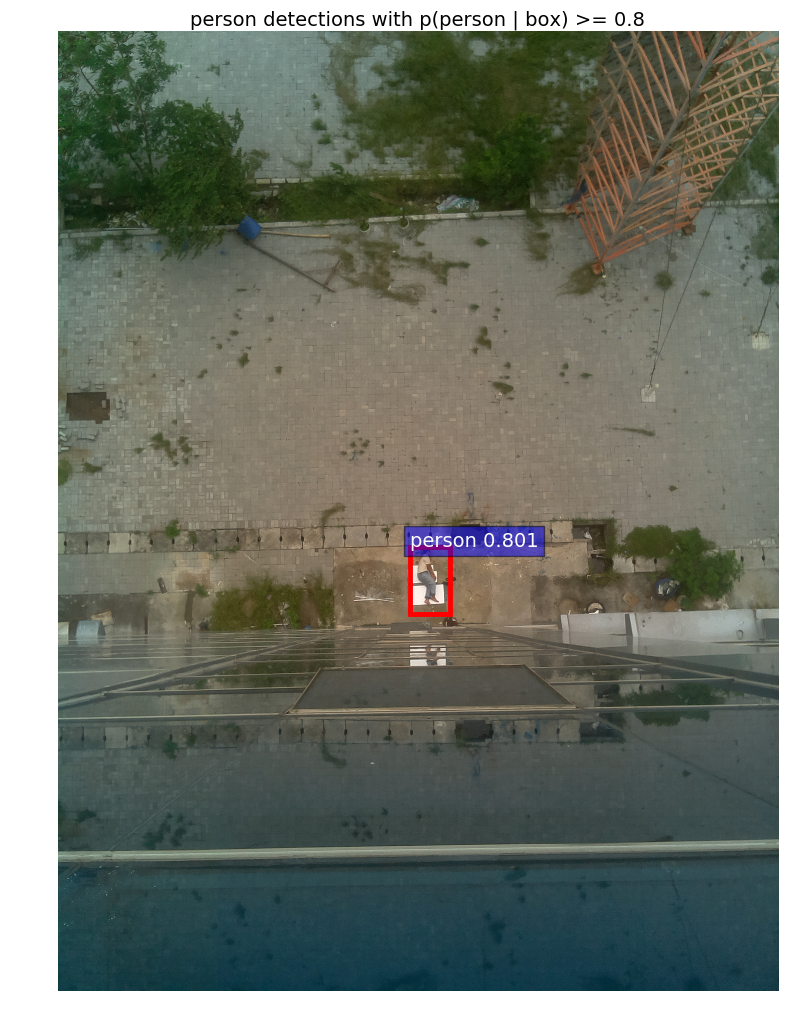
\includegraphics[width=\textwidth]{6}
    \caption{}
  \end{subfigure}
  \caption{Hasil Pengujian Deteksi Berbagai Sikap dan Ketinggian }
  \label{fig:korban_bencana_tinggi}
\end{figure}

Total gambar yang diambil sebanyak 152 gambar terdiri dari 78 gambar landscape dan sisanya potrait dengan masing masing 18 gambar untuk setiap resolusi. Dari 152 gambar tersebut, terdeteksi sebanyak 33 gambar potrait atau $11,84\%$ dari total gambar potrait dan 9 gambar landscape atau $43,42\%$ dari total gambar landscape. Dalam Gambar~\ref{fig:korban_bencana_tinggi} disajikan beberapa gambar yang mewakili hasil dari deteksi. Pada baris pertama terdapat gambar potrait pada lantai 1 dalam pose (a) terlentang, (b) miring dan (c) tertutup sebagian. Pada baris kedua terdapat gambar (d) potrait pada lantai 3 dalam pose terlentang, (e) landscape pada lantai 1 dalam pose terlentang dan (f) potrait pada lantai 4 dalam pose miring.

\begin{table}[ht]
\centering
\caption{Jumlah Gambar Terdeteksi Berdasarkan Resolusi}
\label{table:detectbyres}
\resizebox{\textwidth}{!}{%
\begin{tabular}[\textwidth] { c c c c | c c c c c c}
\hline 
Resolusi & \multicolumn{2}{c}{Rata Rata} & Jumlah & \multicolumn{6}{c}{Ketinggian (m)}\\
(WxH) & Waktu (s) & Proposal &  Terdeteksi & 5,4 & 9,7 &  14 & 18,3 & 22,6 & 26,9 \\
\hline

640x480& 0,0379210526& 229 & 1 &  &  &  &  &  \\
480x640& & &4& 3 & 1 &  &  &  &  \\
\hline
800x600& 0,0411578947 & 255 & 2& 1 & &  & & &1 \\
600x800& & &9 & 3 & 2 &  1 & 2 &  & 1\\
\hline
1296x972& 0,0534210526 & 268 & 3 & 2 &  &  & 1 & & \\
972x1296& & & 9&   3 & 2 & 1 & 1& 1& 1\\
\hline
2592x1944& 0,1061578947 & 254 & 3 & 1  &  &  &  1& & 1 \\
1944x2592& & & 11&  3 & 1 & 2 &2 &1 &2 \\
\hline 
\end{tabular} }
\end{table}

Hasil proses deteksi disajikan pada Tabel~\ref{table:detectbyres} dimana terdapat rata rata waktu yang dibutuhkan, banyaknya proposal, total terdeteksi dan jumlah terdeteksinya gambar pada varian ketinggian untuk masing masing resolusi. Proposal yang dimaksud adalah banyaknya kemungkinan ketika pada proses RPN. Jumlah terdeteksi yang dimaksud adalah jumlah gambar yang terdeteksi, dimana jika mendapatkan nilai tiga pada suatu ketinggian artinya ketiga pose dapat dideteksi. Ketinggian dalam meter merepresentasikan ketinggian yang ada pada lantai 1 hingga 6.

Dari tabel tersebut, dapat dilihat bahwa kecepatan deteksi setiap gambar paling cepat pada resolusi terendah yaitu 640x480 dengan waktu 0,0379210526 detik dan paling lama pada resolusi tertinggi 2592x1944 dengan waktu 0,1061578947 detik. Hal ini akan sangat berpengaruh terhadap waktu yang digunakan jika dilakukan deteksi pada gambar yang sangat banyak. Resolusi tertinggi memberikan hasil deteksi terbaik dibandingkan resolusi lainnya, walaupun tidak terlalu signifikan pada resolusi 800x600 dengan 1296x972.